%Preamble
\documentclass[12pt]{article}
\usepackage{fancyhdr}
\usepackage{extramarks}
\usepackage{amsmath}
\usepackage{amssymb}
\usepackage{amsthm}
\usepackage{amsrefs}
\usepackage{amsfonts}
\usepackage{mathrsfs}
\usepackage{mathtools}
\usepackage[mathcal]{eucal} %% changes meaning of \mathcal
\usepackage{enumerate}
\usepackage[shortlabels]{enumitem}
\usepackage{verbatim} %% includes comment environment
\usepackage{hyperref}
\usepackage[capitalize]{cleveref}
\crefformat{equation}{~(#2#1#3)}
\usepackage{caption, subcaption}
\usepackage{graphicx}
\usepackage{fullpage} %%smaller margins
\usepackage[all,arc]{xy}
\usepackage{mathrsfs}

\hypersetup{
    linktoc=all,     % set to all if you want both sections and subsections linked
}

\topmargin=-0.45in
\evensidemargin=0in
\oddsidemargin=0in
\textwidth=6.5in
\textheight=9.0in
\headsep=0.25in
\setlength{\headheight}{16pt}

\linespread{1.0}

\pagestyle{fancy}
\lhead{\Name}
\chead{\hwClass: \hwTitle}
\rhead{\hwDueDate}
\lfoot{\lastxmark}
\cfoot{\thepage}

\renewcommand\headrulewidth{0.4pt}
\renewcommand\footrulewidth{0.4pt}

\setlength\parindent{0pt}

%% Title Info
\newcommand{\hwTitle}{HW \# 5}
\newcommand{\hwDueDate}{March 1, 2021}
\newcommand{\hwClass}{AMATH 585}
\newcommand{\hwClassTime}{}
\newcommand{\hwClassInstructor}{}
\newcommand{\Name}{\textbf{Marlin Figgins}}


%% MATH MACROS
\newcommand{\bbF}{\mathbb{F}}
\newcommand{\bbN}{\mathbb{N}}
\newcommand{\bbQ}{\mathbb{Q}}
\newcommand{\bbR}{\mathbb{R}}
\newcommand{\bbZ}{\mathbb{Z}}
\newcommand{\bbC}{\mathbb{C}}
\newcommand{\abs}[1]{ \left| #1 \right| }
\newcommand{\diff}[2]{\frac{d #1}{d #2}}
\newcommand{\infsum}[1]{\sum_{#1}^{\infty}}
\newcommand{\norm}[1]{ \left|\left| #1 \right|\right| }
\newcommand{\eval}[1]{ \left. #1 \right| }
\newcommand{\Expect}[1]{\mathbb{E}\left[#1 \right]}
\newcommand{\Var}[1]{\mathbb{V}\left[#1 \right]}
\renewcommand{\vec}[1]{\mathbf{#1}}

\renewcommand{\phi}{\varphi}
\renewcommand{\emptyset}{\O}

%--------Theorem Environments--------
%theoremstyle{plain} --- defaultx
\newtheorem{thm}{Theorem}[section]
\newtheorem{cor}[thm]{Corollary}
\newtheorem{prop}[thm]{Proposition}
\newtheorem{lem}[thm]{Lemma}
\newtheorem{conj}[thm]{Conjecture}
\newtheorem{quest}[thm]{Question}

\theoremstyle{definition}
\newtheorem{defn}[thm]{Definition}
\newtheorem{defns}[thm]{Definitions}
\newtheorem{con}[thm]{Construction}
\newtheorem{exmp}[thm]{Example}
\newtheorem{exmps}[thm]{Examples}
\newtheorem{notn}[thm]{Notation}
\newtheorem{notns}[thm]{Notations}
\newtheorem{addm}[thm]{Addendum}

% Environments for answers and solutions
\newtheorem{exer}{Exercise}
\newtheorem{sol}{Solution}

\theoremstyle{remark}
\newtheorem{rem}[thm]{Remark}
\newtheorem{rems}[thm]{Remarks}
\newtheorem{warn}[thm]{Warning}
\newtheorem{sch}[thm]{Scholium}

\makeatletter
\let\c@equation\c@thm
\makeatother

\begin{document}
\begin{exer}
    The key to efficiency in the \verb+chebfun+ package, which you used in a previous homework
exercise, is the ability to rapidly translate between the values of a function at the
Chebyshev points, $\cos ( \pi j/n )$, $j=0, \ldots , n$, and the coefficients $a_0 , \ldots , a_n$,
in a Chebyshev expansion of the function's $n$th-degree polynomial interpolant:
$p(x) = \sum_{j=0}^n a_j T_j (x)$, where $T_j (x) = \cos ( j \arccos (x) )$ is the $j$th
degree Chebyshev polynomial.  Knowing the coefficients $a_0 , \ldots , a_n$, one can evaluate
$p$ at the Chebyshev points by evaluating the sums
\begin{equation}
p ( \cos ( k \pi / n ) ) = \sum_{j=0}^n a_j \cos ( j k \pi / n ) ,~~~k=0, \ldots , n.
\label{Cheby}
\end{equation}
These sums are much like the real part of the sums in the FFT,
\[
F_k = \sum_{j=0}^{n-1} e^{2 \pi i j k / n} f_j ,~~~k=0, \ldots , n-1 ,
\]
but the argument of the cosine differs by a factor of $2$ from the values that would make
them equal.  Explain how the FFT or a closely related procedure could be used to evaluate
the sums in (\ref{Cheby}).  To go in the other direction, and efficiently determine the coefficients
$a_0 , \ldots , a_n$ from the function values $f( \cos ( k \pi / n ) )$, what method would you use?

\end{exer}

\begin{sol}
    Writing the input $f_{j}$ as a vector $\vec{f}$ with elements
     \begin{align*}
         f_{j} = e^{- \pi i j k / n} a_{j},
    \end{align*}
    we see that
    \begin{align*}
        F_{k}(\vec{f}) = \sum_{j=0}^{n-1} a_{j} e^{\pi i jk / n}.
    \end{align*}
    Taking the real part of this quantity
    \begin{align*}
        \Re[F_{k}(\vec{f})] = \sum_{j=0}^{n-1} a_{j} \cos( \pi jk / n ) = p(\cos(k \pi / n)) - a_{n}\cos(k\pi)
    \end{align*}
    We can re-arrange this as
    \begin{align*}
        p(\cos(k\pi) / n) = a_{n} \cos(k \pi) + F_{k}(\vec{f}),
    \end{align*}
    with $\vec{f}$ as defined above. With the substitution defined as above, we can use the FFT to compute the values defined in (\ref{Cheby}). Going backwards, starting with the function values $ p(\cos(k\pi) / n)$ would require taking the inverse FFT of 
    \begin{align*}
        p(\cos(k\pi) / n) - a_{n} \cos(k \pi) = F_{k}(\vec{f}).
    \end{align*}
    This would allows us to recover $\vec{f}$ and therefore the coefficients $a_{i}$ as we know how they are scaled to get the $f_{i}$.
  \end{sol}

\newpage

\begin{exer}
      On the course web page
is a finite difference code (steady2d.m) to solve the boundary value
problem:
\[
\frac{\partial}{\partial x} \left( a(x,y) \frac{\partial u}{\partial x}
\right) +
\frac{\partial}{\partial y} \left( a(x,y) \frac{\partial u}{\partial y}
\right) = f(x,y)~~~\mbox{in } (0,1) \times (0,1)
\]
\[
u(x,0) = u(x,1) = u(0,y) = u(1,y) = 0 ,
\]
where $a(x,y) = 1 + x^2 + y^2$ and $f(x,y) = 1$.
It uses a direct solver for the linear system.

Replace this direct solver first by the Jacobi method, then by the Gauss
Seidel method, and then by the SOR method.
For each method, make a plot of the relative residual norm,
$\| b - A u^k \| / \| b \|$ versus iteration number $k$.
(Use a logarithmic scale for the residual; i.e., you may use \verb+semilogy+
in Matlab to do the plot.)
Try several different values for the parameter $\omega$ in SOR,
until you find one that seems to work well.

Then try solving the linear system using the conjugate gradient
method.  You may write your own CG code or use the one in Matlab
(called {\bf pcg}).  First try CG without a preconditioner
(i.e., with preconditioner equal to the identity) and then try CG
with the Incomplete Cholesky decomposition as the preconditioner.
You may use \verb+ichol+ in Matlab to generate the incomplete Cholesky 
decomposition.  Again make a plot of relative residual norm versus 
iteration number for the CG method.

Experiment with a few different mesh sizes and comment on how the
number of iterations required to reach a fixed level of accuracy
seems to vary with $h$ for each method.

\end{exer}

\begin{sol}
    I implemented all solvers in julia. The code for which can be found attached in the appendix. I also present two plots. One showing the relative residual norms of different methods assuming the same starting vector $\vec{u}_{0}$ and a fixed matrix $\vec{A}$ of size $N^2 \times N^2$.

    %TODO: Analyze results.

    \begin{figure}[h]
        \centering
        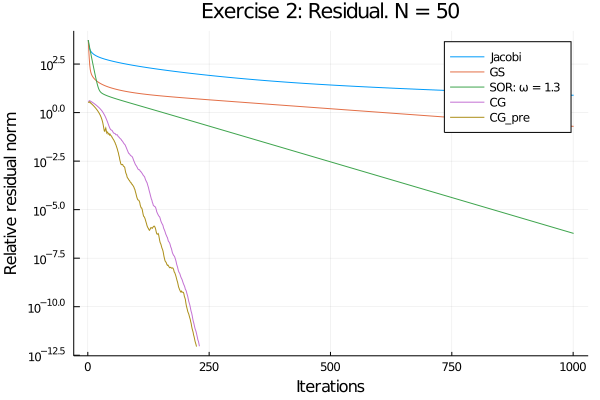
\includegraphics[width=0.8\linewidth]{figs/hw-5-exer-2-residual.png}
        \caption{Plotting the relative residual norm for various iterative methods.}%
        \label{fig:E2-res}
    \end{figure}

    \begin{figure}[h]
        \centering
        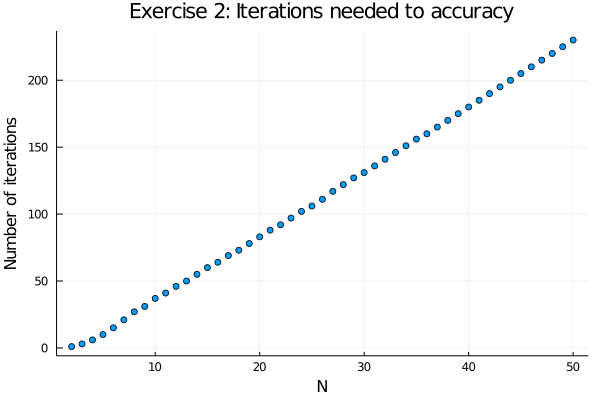
\includegraphics[width=0.8\linewidth]{figs/hw-5-exer-2-iterations-needed.png}
        \caption{Plotting the relative residual norm for various iterative methods.}%
        \label{fig:E2-iter}
    \end{figure}

\end{sol}

\newpage
 \
 \newpage

\begin{exer}
    Suppose a symmetric positive definite matrix $A$ has one thousand eigenvalues
uniformly distributed between $1$ and $10$, and one eigenvalue of $10^4$.
Suppose another symmetric positive definite matrix $B$ has an eigenvalue
of $1$ and has one thousand eigenvalues uniformly distributed between $10^3$
and $10^4$.
Since each matrix has condition number $\kappa = 10^4$, we have seen
that the error at step $k$ of the CG algorithm satisfies
\[
\frac{\| e^{(k)} \|_{A,B}}{\| e^{(0)} \|_{A,B}} \leq 2 \left( \frac{
\sqrt{\kappa} - 1}{\sqrt{\kappa} +1} \right)^k = 2 \left( \frac{99}{101} 
\right)^k .
\]
Give another bound on $\| e^{(k)} \|_A / \| e^{(0)} \|_A$ based
on a polynomial that is a product of a degree $k-1$ Tchebyshev polynomial
on the interval $[1,10]$ and a linear polynomial that is $1$ at the
origin and $0$ at $10^4$.  Give another bound on $\| e^{(k)} \|_B /
\| e^{(0)} \|_B$ based on a polynomial that is a product of a degree $k-1$ 
Tchebyshev polynomial on the interval $[ 10^3 , 10^4]$ and a linear polynomial
that is $1$ at the origin and $0$ at $1$.  For which matrix would you
expect CG to converge more rapidly?  [If you are not sure, you may try
it in Matlab.]
\end{exer}

\begin{sol}
    By exhibiting a polynomial $p_{k}$ which is small near the cluster of eigenvalues and small near the outlier eigenvalue, we can bound $\norm{e^{(k)}}_{A, B}$. Given a polynomial $p(x)$, we have that
    \begin{align*}
        \norm{P(A) e^{(0)}}_{A} \leq \norm{e^{0}}_{A} \max_{1\leq j\leq m} \norm{P(\lambda_{j})}.
    \end{align*}
Let $[\lambda_{a}, \lambda_{b}]$ be the interval where the eigenvalues are clustered and $\lambda_{o}$ is the outlier eigenvalue and $\epsilon>0$. Starting with the example for which $\lambda_{1} = 1$ and $\lambda_{m} = 10$ and $\lambda_{o} = 10000$, we have that
\begin{align*}
    \norm{P(A) e^{(0)}}_{A} \leq \norm{ e^{(0)} }_{A} \max_{\lambda_{a} < \lambda < \lambda_{b}} \norm{P_{k}(\lambda)} 
\end{align*}
if we have that $P_{k}(\lambda_{0}) = 0$. Additionally, we make sure that $P_{k}$ is near 0 where our eigenvalue clusters. Suppose that we have $k - 1 < N$ clusters of width $\epsilon$ where $N$ is the number of the eigenvalues. Then, we can refine our estimate as 
\begin{align*}
    \frac{\norm{P_k(A) e^{(0)}}_{A}}{\norm{ e^{(0)} }_{A}}  \leq \max_{\lambda \in (\lambda_{i} - \epsilon, \lambda_{i} + \epsilon),1\leq i \leq k} \norm{P_{k}(\lambda)}. 
\end{align*}
We can then write the $k$-degree polynomial as
\begin{align*}
    P_{k}(\lambda) = \left(\prod_{i=1}^{k-1} \lambda_{i}\right)^{-1} \left( \prod_{x=1}^{k-1} (\lambda_{i} - \lambda)\right) \left(\frac{\lambda_{o} - \lambda}{\lambda_{o}}\right).
\end{align*}
In our case, with one cluster, we have that
\begin{align*}
    \max_{\abs{\lambda_{1} - \lambda} < \epsilon} \norm{P_{2}} &= \max_{\abs{\lambda_{1} - \lambda} < \epsilon}  \abs{\frac{(\lambda_{1} - \lambda)(\lambda_{o} - \lambda)}{\lambda_{1} \lambda_{o}} }\\
                                                               &= \abs{ \frac{(\lambda_{1} - (\lambda_{1} - \epsilon)) (\lambda_{o} - (\lambda_{1} - \epsilon)) }{\lambda_{1}\lambda_{o}}}\\
                                                               &= \frac{\epsilon (\lambda_{o} - \lambda_{1} + \epsilon)}{\lambda_{1}\lambda_{0}},
\end{align*}
where I've assumed  that $\lambda_{o} > \lambda_{1} - \epsilon$. This is on order of $\epsilon$ so as the size of the grouping shrinks, we see that the
\begin{align*}
    \frac{\norm{P_2(A) e^{(0)}}_{A}}{\norm{ e^{(0)} }_{A}}  \text{ is of order } O(\epsilon).
\end{align*}
This gives one step bound for $A$ like
\begin{align*}
    \frac{\norm{e^{(2)}}_{A}}{\norm{ e^{(0)} }_{A}} \leq 0.8.
\end{align*}
Repeating, this process for higher $k$ will produce a polynomial which is approximately flat on the region $(\lambda_{i} - \epsilon, \lambda_{i} + \epsilon)$. In the case of matrix $A$, we can try to tile the region $[1, 10]$ with $k-1$ evenly spaced intervals to speed up convergence. This will give a better bound on the rate of convergence. In the case of matrix $B$ for which the region is $[10^{3}, 10^{4}]$ we have that $\lambda_{o} \ll \lambda_{a}$, so there should be a sign flip in the derivation of $\max \norm{P_{2}}$. Regardless, we can use the formula derived to get an intuition on which matrix will be quicker to solve. My guess is that matrix $A$ will be easier to solve since $\epsilon$ is much smaller so fewer intervals are needed to cover $[\lambda_{a}, \lambda_{b}]$ i.e. a lower value of $k$ is needed to cover the interval with the main cluster of the eigenvalues. 
\end{sol} 
\end{document}
